% ======================================================================
%  Chapter 5 — Geometry of Maxwell Bands
%  derived for electromagnetic modes with the correct inner product.
% ======================================================================

\section{Phase geometry in parameter space}
\label{sec:ch5-phase-geometry}

The photonic band structure $\omega_n(\kvec)$ is an eigenvalue problem
parametrised by the Bloch wavevector $\kvec$.  As $\kvec$ changes
continuously, the eigenfrequency $\omega_n$ changes smoothly (unless
bands cross), and the eigenmode $\mathbf{u}_{n\kvec}(\rvec)$
also evolves smoothly---up to a \emph{phase}.

The eigenvalue equation determines $\mathbf{u}_{n\kvec}$ only up to a
$\kvec$-dependent phase factor:
$\mathbf{u}_{n\kvec}\to\ee^{\ii\chi_n(\kvec)}\mathbf{u}_{n\kvec}$ is
equally valid for any smooth real function $\chi_n(\kvec)$.  This is a
gauge freedom, precisely analogous to the gauge freedom of the vector
potential in electromagnetism.

The Berry connection, Berry curvature, and Chern number are the
mathematical objects that describe the geometry of this gauge freedom
\cite{raghu2008analogs,zhao2020first,lee2022calculation}.
They are the central tools of topological band theory.  In this chapter,
we derive them from the Maxwell eigenproblem using the electromagnetic
inner product established in \chref{ch:normal-modes}.

\section{Berry connection for Maxwell modes}
\label{sec:ch5-berry-connection}

\subsection{Definition}
\label{sec:ch5-bc-definition}

Consider a single nondegenerate band $n$ with cell-periodic Bloch
eigenmode $\mathbf{u}_{n\kvec}(\rvec)$, normalised so that
$\eip{\mathbf{u}_{n\kvec}}{\mathbf{u}_{n\kvec}}=1$ using the dispersive
energy inner product \eqref{eq:ch3-disp-norm}.

\begin{definition}[Electromagnetic Berry connection]
  \label{def:ch5-berry-connection}
  The Berry connection of the $n$-th Maxwell band is the one-form on
  the Brillouin zone defined by
  \begin{equation}\label{eq:ch5-berry-connection}
    \boxed{%
    \Aberryvec_n(\kvec)
    = \ii\,\frac{
      \displaystyle\int_\Omega
      \mathbf{u}_{n\kvec}^\dagger(\rvec)\,
      \Mgmat(\rvec,\omega_{n\kvec})\,
      \nabla_\kvec\mathbf{u}_{n\kvec}(\rvec)\,\dd^d r
    }{
      \displaystyle\int_\Omega
      \mathbf{u}_{n\kvec}^\dagger(\rvec)\,
      \Mgmat(\rvec,\omega_{n\kvec})\,
      \mathbf{u}_{n\kvec}(\rvec)\,\dd^d r
    }\,.}
  \end{equation}
  With our normalisation convention, the denominator equals unity and
  the Berry connection simplifies to
  \begin{equation}\label{eq:ch5-berry-connection-normalised}
    \Aberryvec_n(\kvec)
    = \ii\int_\Omega
    \mathbf{u}_{n\kvec}^\dagger\,
    \Mgmat\,
    \nabla_\kvec\mathbf{u}_{n\kvec}\,\dd^d r\,.
  \end{equation}
\end{definition}

\begin{remark}
  In the nondispersive limit, $\Mgmat\to\Mmat$ and the Berry connection
  reduces to
  $\Aberryvec_n=\ii\int_\Omega\mathbf{u}_n^\dagger\Mmat
  \nabla_\kvec\mathbf{u}_n\,\dd^d r$.  In the energy-weighted
  representation $\emfieldw_n=\Mgmat^{1/2}\mathbf{u}_n$, it takes the
  familiar quantum-mechanical form
  $\Aberryvec_n=\ii\int_\Omega\emfieldw_n^\dagger
  \nabla_\kvec\emfieldw_n\,\dd^d r$.
\end{remark}

\subsection{Reality of the Berry connection}
\label{sec:ch5-bc-real}

\begin{proposition}
  The Berry connection $\Aberryvec_n(\kvec)$ is real-valued for each
  component $\alpha$: $\Aberry_{n,\alpha}\in\mathbb{R}$.
\end{proposition}

\begin{proof}
Work with the energy-weighted Bloch function
$\emfieldw_n(\rvec,\kvec)=\Mgmat^{1/2}(\rvec)\,\mathbf{u}_{n\kvec}(\rvec)$
introduced in \secref{sec:ch3-energy-weighted}, which satisfies the standard
normalisation $\int_\Omega\emfieldw_n^\dagger\emfieldw_n\,\dd^d r=1$.
From the definition \eqref{eq:ch5-berry-connection}, one can express the Berry
connection entirely in terms of $\emfieldw_n$:
\begin{equation}\label{eq:ch5-berry-weighted}
  \Aberry_{n,\alpha}
  = \ii\int_\Omega\emfieldw_n^\dagger(\rvec,\kvec)\,
  \nabla_{k_\alpha}\emfieldw_n(\rvec,\kvec)\,\dd^d r\,.
\end{equation}
Now differentiate the normalisation condition with respect to $k_\alpha$:
\begin{equation}\label{eq:ch5-norm-deriv}
  \nabla_{k_\alpha}\int_\Omega
  \emfieldw_n^\dagger\,\emfieldw_n\,\dd^d r
  = \nabla_{k_\alpha}(1) = 0\,.
\end{equation}
Expanding the left-hand side:
\begin{equation}
  \int_\Omega\bigl(
    \nabla_{k_\alpha}\emfieldw_n^\dagger\;\emfieldw_n
    + \emfieldw_n^\dagger\;\nabla_{k_\alpha}\emfieldw_n
  \bigr)\dd^d r = 0\,.
\end{equation}
The second term is $-\ii\Aberry_{n,\alpha}$ by
\eqref{eq:ch5-berry-weighted}, and its complex conjugate gives the
first term as $+\ii\Aberry_{n,\alpha}^*$.  Therefore
\begin{equation}
  \ii\Aberry_{n,\alpha}^* - \ii\Aberry_{n,\alpha} = 0\,,
  \qquad\text{i.e.}\quad
  \Aberry_{n,\alpha}^* = \Aberry_{n,\alpha}\,.
\end{equation}
Hence $\Aberry_{n,\alpha}\in\mathbb{R}$ for every component $\alpha$.
\end{proof}

\begin{remark}
If one works directly with the cell-periodic eigenmode $\mathbf{u}_n$
and the $\Mgmat$-weighted inner product, an extra term
$\int\mathbf{u}_n^\dagger\,\nabla_{k_\alpha}\Mgmat\,\mathbf{u}_n\,\dd^d r$
appears from the $\kvec$-dependence of $\Mgmat$ through
$\omega_n(\kvec)$.  This term vanishes after absorbing the metric into
the field via $\emfieldw_n=\Mgmat^{1/2}\mathbf{u}_n$.  The
energy-weighted formulation is therefore the natural setting for
defining the Berry connection \cite{gangaraj2016berry,silveirinha2016bulk},
and is the convention we adopt
throughout this book.
\end{remark}

\subsection{Gauge transformation}
\label{sec:ch5-gauge}

Under a gauge transformation
$\mathbf{u}_{n\kvec}\to\ee^{\ii\chi_n(\kvec)}\mathbf{u}_{n\kvec}$:
\begin{equation}\label{eq:ch5-gauge-transform}
  \Aberryvec_n(\kvec) \;\to\;
  \Aberryvec_n(\kvec) - \nabla_\kvec\chi_n(\kvec)\,.
\end{equation}
This is exactly the gauge transformation of the electromagnetic vector
potential $\mathbf{A}\to\mathbf{A}-\nabla\Lambda$.  The Berry
connection is a \emph{connection} on a $\mathrm{U}(1)$ bundle over the
Brillouin zone, and its gauge dependence is the defining property of a
connection.

\section{Berry curvature}
\label{sec:ch5-curvature}

\begin{definition}[Berry curvature]
  \label{def:ch5-berry-curvature}
  The Berry curvature is the curl of the Berry connection:
  \begin{equation}\label{eq:ch5-berry-curvature}
    \boxed{%
    \Fberryvec_n(\kvec) = \nabla_\kvec\times\Aberryvec_n(\kvec)\,.}
  \end{equation}
  In two dimensions (the $k_x$--$k_y$ plane), only the $z$-component
  is nonzero:
  \begin{equation}\label{eq:ch5-curvature-2d}
    \Omega_n(\kvec)
    = \pderiv{\Aberry_{n,y}}{k_x} - \pderiv{\Aberry_{n,x}}{k_y}\,.
  \end{equation}
\end{definition}

\begin{proposition}[Gauge invariance]
  The Berry curvature is gauge-invariant \cite{raman2010photonic}:
  \begin{equation}
    \Omega_n(\kvec) \;\to\; \Omega_n(\kvec)
    \qquad\text{under }
    \mathbf{u}_n\to\ee^{\ii\chi}\mathbf{u}_n\,.
  \end{equation}
\end{proposition}

\begin{proof}
From \eqref{eq:ch5-gauge-transform},
$\Aberryvec_n\to\Aberryvec_n-\nabla_\kvec\chi$.  Taking the curl:
$\nabla_\kvec\times(\Aberryvec_n-\nabla_\kvec\chi)
=\nabla_\kvec\times\Aberryvec_n-\nabla_\kvec\times\nabla_\kvec\chi
=\Fberryvec_n-\mathbf{0}=\Fberryvec_n$.
\end{proof}

\subsection{An explicit formula}
\label{sec:ch5-curvature-explicit}

The Berry curvature can also be written without taking derivatives of
the eigenmode, using the second-order perturbation theory formula.
For a nondegenerate band $n$:
\begin{equation}\label{eq:ch5-kubo-formula}
  \Omega_n(\kvec)
  = -2\sum_{m\neq n}
  \frac{
    \imag\bigl[
      \langle\mathbf{u}_n|\partial_{k_x}\Maxop|\mathbf{u}_m\rangle
      \langle\mathbf{u}_m|\partial_{k_y}\Maxop|\mathbf{u}_n\rangle
    \bigr]
  }{
    (\omega_m-\omega_n)^2
  }\,,
\end{equation}
where the matrix elements
$\langle\mathbf{u}_n|\partial_{k_\alpha}\Maxop|\mathbf{u}_m\rangle
\equiv\int\mathbf{u}_n^\dagger(\partial_{k_\alpha}\Maxop)\mathbf{u}_m\,\dd^3r$
use the standard (unweighted) $L^2$ inner product, the modes are
normalised so that $\int\mathbf{u}_n^\dagger\Mmat\mathbf{u}_n\,\dd^3r=1$,
and $\partial_{k_\alpha}\Maxop$ is the velocity operator from the
Hellmann--Feynman formula.  For dispersive media, the normalisation
should use $\Mgmat(\omega_n)$ in place of $\Mmat$.

This ``Kubo-like'' formula shows that the Berry curvature is large when
two bands are \emph{close in frequency} (small $\omega_m-\omega_n$) and
when the velocity-operator matrix element between them is large.  Near a
Dirac point, where two bands touch, the Berry curvature diverges as the
gap is opened by a perturbation---this is the origin of the concentrated
Berry flux near gapped Dirac cones.

\section{Berry phase}
\label{sec:ch5-berry-phase}

The Berry phase is the line integral of the Berry connection around a
closed loop $C$ in the Brillouin zone:
\begin{equation}\label{eq:ch5-berry-phase}
  \gamma_n(C) = \oint_C \Aberryvec_n(\kvec)\cdot\dd\kvec\,.
\end{equation}
By Stokes' theorem (when the Berry connection is smooth inside the
region $S$ enclosed by $C$):
\begin{equation}\label{eq:ch5-berry-stokes}
  \gamma_n(C) = \int_S \Omega_n(\kvec)\,\dd^2 k\,.
\end{equation}
The Berry phase is gauge-invariant modulo $2\pi$: under
$\mathbf{u}_n\to\ee^{\ii\chi}\mathbf{u}_n$, $\gamma_n\to\gamma_n-[\chi]_C$,
where $[\chi]_C$ is the winding of $\chi$ around $C$, which is an
integer multiple of $2\pi$ for a single-valued gauge transformation.

\section{The Chern number}
\label{sec:ch5-chern}

\begin{definition}[Chern number]
  \label{def:ch5-chern}
  The (first) Chern number of the $n$-th band is the integral of the
  Berry curvature over the entire Brillouin zone:
  \begin{equation}\label{eq:ch5-chern}
    \boxed{%
    \Chern_n = \frac{1}{2\pi}\int_\BZ \Omega_n(\kvec)\,\dd^2 k\,.}
  \end{equation}
\end{definition}

\subsection{Quantisation}
\label{sec:ch5-quantisation}

\begin{theorem}[Chern number is an integer]
  \label{thm:ch5-chern-integer}
  When the $n$-th band is nondegenerate (separated from all other bands
  by gaps), $\Chern_n\in\mathbb{Z}$.
\end{theorem}

\begin{proof}[Proof sketch]
The Brillouin zone is a torus $T^2$.  On this compact manifold without
boundary, the eigenmode $\mathbf{u}_{n\kvec}$ defines a $\mathrm{U}(1)$
line bundle.  The Chern number is the first Chern class of this bundle,
which is always an integer by a topological theorem (the integrality of
the first Chern class).

More concretely: cover the torus with two overlapping patches $U_\alpha$
and $U_\beta$.  On each patch, choose a smooth gauge for
$\mathbf{u}_n$.  On the overlap $U_\alpha\cap U_\beta$, the two gauges
are related by a transition function
$g_{\alpha\beta}(\kvec)=\ee^{\ii\chi_{\alpha\beta}(\kvec)}$.  The
Chern number equals the winding number of $g_{\alpha\beta}$ around the
overlap region, which is necessarily an integer:
\begin{equation}
  \Chern_n = \frac{1}{2\pi}\oint_{\partial U_\alpha}
  \nabla_\kvec\chi_{\alpha\beta}\cdot\dd\kvec \;\in\;\mathbb{Z}\,.
\end{equation}
\end{proof}

\subsection{Properties}
\label{sec:ch5-chern-properties}

\begin{enumerate}
  \item \textbf{Topological invariance.}
  $\Chern_n$ cannot change under any smooth deformation of the medium
  $\Mmat(\rvec)\to\Mmat(\rvec)+\delta\Mmat(\rvec)$ that does not close
  the band gap above or below band $n$.  A change in $\Chern_n$
  requires a gap closing (a topological phase transition).

  \item \textbf{Sum rule.}
  The sum of Chern numbers over all bands is zero:
  $\sum_n\Chern_n=0$.  This follows from the fact that the total Berry
  curvature summed over all bands vanishes identically at every $\kvec$.

  \item \textbf{Gap Chern number.}
  For a band gap between bands $n$ and $n+1$, define the gap Chern
  number as $\Chern_{\mathrm{gap}}=\sum_{j=1}^{n}\Chern_j$.  This is
  the quantity that determines the number and direction of edge states
  in the gap.
\end{enumerate}

\section{Symmetry constraints on Berry curvature and Chern number}
\label{sec:ch5-symmetry}

\subsection{Time-reversal symmetry}
\label{sec:ch5-tr}

\begin{proposition}
  If the Maxwell system is time-reversal invariant, the Berry curvature
  satisfies
  \begin{equation}\label{eq:ch5-tr-curvature}
    \Omega_n(\kvec) = -\Omega_n(-\kvec)\,.
  \end{equation}
\end{proposition}

\begin{proof}
Time reversal maps $\mathbf{u}_{n\kvec}$ to $\Top\mathbf{u}_{n\kvec}$
at $-\kvec$.  Using the explicit action
$\Top\mathbf{u}=\sigma_z\mathbf{u}^*$ and the TR condition on $\Mmat$
(\eqref{eq:ch2-TR-condition}):
\begin{align}
  \Aberry_{n,\alpha}(-\kvec)
  &= \ii\int(\Top\mathbf{u}_n)^\dagger\Mgmat\,
    \nabla_{(-k_\alpha)}(\Top\mathbf{u}_n)\,\dd^d r \notag\\
  &= \ii\int\mathbf{u}_n^T\sigma_z\Mgmat\,
    (-\nabla_{k_\alpha})(\sigma_z\mathbf{u}_n^*)\,\dd^d r \notag\\
  &= -\Aberry_{n,\alpha}(\kvec) + \nabla_{k_\alpha}\phi_n(\kvec)\,,
\end{align}
where $\phi_n$ is a gauge-dependent phase.  Taking the curl eliminates
$\phi_n$ and gives $\Omega_n(-\kvec)=-\Omega_n(\kvec)$.
\end{proof}

\begin{corollary}
  Under time-reversal symmetry, $\Chern_n=0$
\cite{kane2005cond}.
\end{corollary}

\begin{proof}
$\Chern_n=(2\pi)^{-1}\int_\BZ\Omega_n(\kvec)\,\dd^2k$.
Since the BZ is symmetric under $\kvec\to-\kvec$ and
$\Omega_n(\kvec)=-\Omega_n(-\kvec)$, the integrand is odd and the
integral vanishes.
\end{proof}

This is the fundamental reason why \emph{nonreciprocal media are
required for nonzero photonic Chern numbers}.  Without breaking
time-reversal symmetry, the Berry curvature integrates to zero and
there are no topologically protected one-way edge states.

\subsection{Inversion symmetry}
\label{sec:ch5-inversion}

Under inversion ($\Pop$):
\begin{equation}\label{eq:ch5-inv-curvature}
  \Omega_n(\kvec) = \Omega_n(-\kvec)\,.
\end{equation}
Combined with time reversal, $\Omega_n(\kvec)=-\Omega_n(-\kvec)
=\Omega_n(-\kvec)$, so $\Omega_n(\kvec)=0$ at every $\kvec$---the
Berry curvature vanishes identically when both $\Top$ and $\Pop$ are
present.

\subsection{Breaking time reversal: the gyrotropic case}
\label{sec:ch5-breaking-tr}

When the gyrotropic parameter $\kappa\neq 0$, time reversal is broken
and the constraint $\Omega_n(\kvec)=-\Omega_n(-\kvec)$ no longer holds.
The Berry curvature can be nonzero and can integrate to a nonzero
Chern number.  How this happens in detail---through the gap opening at
Dirac points---is the subject of \chref{ch:dirac-cones} and
\chref{ch:breaking-tr}.

\section{Non-Abelian Berry connection for degenerate bands}
\label{sec:ch5-non-abelian}

When $p$ bands $n_1,\ldots,n_p$ are degenerate or form an isolated
group (separated from all other bands by gaps but possibly touching
each other), the Berry connection becomes a matrix-valued one-form.

\begin{definition}[Non-Abelian Berry connection]
  Define the $p\times p$ matrix
  \begin{equation}\label{eq:ch5-non-abelian-connection}
    [\boldsymbol{\mathcal{A}}_\alpha(\kvec)]_{nm}
    = \ii\int_\Omega
    \mathbf{u}_{n\kvec}^\dagger\,\Mgmat\,
    \pderiv{\mathbf{u}_{m\kvec}}{k_\alpha}\,\dd^d r\,,
    \qquad n,m\in\{n_1,\ldots,n_p\}\,.
  \end{equation}
\end{definition}

The non-Abelian Berry curvature is
\begin{equation}\label{eq:ch5-non-abelian-curvature}
  \mathbf{F}_{\alpha\beta}
  = \pderiv{\boldsymbol{\mathcal{A}}_\beta}{k_\alpha}
  - \pderiv{\boldsymbol{\mathcal{A}}_\alpha}{k_\beta}
  + \ii[\boldsymbol{\mathcal{A}}_\alpha,
       \boldsymbol{\mathcal{A}}_\beta]\,,
\end{equation}
where the commutator term is absent in the Abelian (single-band) case.

The \emph{composite Chern number} of the group of bands is
\begin{equation}\label{eq:ch5-composite-chern}
  \Chern_{\mathrm{composite}}
  = \frac{1}{2\pi}\int_\BZ \Tr\,\mathbf{F}_{xy}\,\dd^2 k\,,
\end{equation}
which is again an integer.

\section{Wilson loops and the Zak phase}
\label{sec:ch5-wilson}

An alternative characterisation of band topology that avoids the need
for a smooth gauge is the \emph{Wilson loop}
\cite{lu2026universal,hsieh2008topological,atala2013direct}.

\begin{definition}[Wilson loop]
  For a closed path $C$ in the Brillouin zone, the Wilson loop is the
  path-ordered exponential of the non-Abelian Berry connection:
  \begin{equation}\label{eq:ch5-wilson-loop}
    \Wloop(C) = \mathcal{P}\exp\biggl(
      -\ii\oint_C \boldsymbol{\mathcal{A}}(\kvec)\cdot\dd\kvec
    \biggr)\,,
  \end{equation}
  where $\mathcal{P}$ denotes path ordering.
\end{definition}

For a single band, the Wilson loop reduces to
$\Wloop=\ee^{-\ii\gamma_n}$, where $\gamma_n$ is the Berry phase.

\paragraph{The Zak phase.}
In one dimension, or for a path that crosses the Brillouin zone in one
direction (say $k_x$ from $-\pi/a$ to $\pi/a$ at fixed $k_y$), the
Berry phase of a single band is called the \emph{Zak phase}:
\begin{equation}\label{eq:ch5-zak}
  \Zak = \int_{-\pi/a}^{\pi/a}\Aberry_{n,x}(k_x)\,\dd k_x\,.
\end{equation}
The Zak phase is quantised to $0$ or $\pi$ (modulo $2\pi$) when the
system has both time-reversal and inversion symmetry, and it
characterises the one-dimensional topological phases discussed in
\chref{ch:one-dimension}.

\paragraph{Wilson-loop winding.}
For a set of bands, the eigenvalues of the Wilson loop matrix
$\Wloop(k_y)$ as a function of $k_y$ trace out curves whose winding
number equals the Chern number of the band group.  This provides a
numerically robust, gauge-invariant method for computing Chern numbers
that we will exploit in \chref{ch:computing-chern}.

\section{Physical meaning of Berry curvature}
\label{sec:ch5-physical}

The Berry curvature is not merely a mathematical construct; it has
direct physical consequences.

\paragraph{Anomalous velocity.}
In a slowly varying potential, a wave packet in band $n$ acquires a
transverse velocity proportional to the Berry curvature:
\begin{equation}\label{eq:ch5-anomalous}
  \dot{\rvec} = \nabla_\kvec\omega_n
  + \dot{\kvec}\times\Fberryvec_n(\kvec)\,.
\end{equation}
The second term is the \emph{anomalous velocity}, analogous to the
Lorentz force but arising from the momentum-space geometry rather than
a real magnetic field
\cite{kane2005sub}.  It is the mechanism behind the photonic Hall
effect and the transverse displacement of light beams in
topological media.

\paragraph{Effective magnetic field in $\kvec$-space.}
The Berry curvature acts as an effective magnetic field in momentum
space.  A concentrated ``Berry monopole'' at a band degeneracy point is
the momentum-space analog of a magnetic monopole.  The Chern number
counts the net monopole charge enclosed by the Brillouin-zone torus.

\paragraph{Bulk-edge correspondence (preview).}
The most dramatic physical consequence of a nonzero Chern number is the
\emph{bulk-edge correspondence}: at an interface between two media with
different gap Chern numbers $\Chern_{\mathrm{gap}}^L$ and
$\Chern_{\mathrm{gap}}^R$, the number of unidirectional edge modes
crossing the gap is
\begin{equation}\label{eq:ch5-bulk-edge}
  N_{\mathrm{edge}} = \Chern_{\mathrm{gap}}^L - \Chern_{\mathrm{gap}}^R\,.
\end{equation}
We will derive this correspondence in detail in \chref{ch:one-way-interface}.

\section{Anomalous velocity and semiclassical dynamics}
\label{sec:ch5-anomalous-velocity}

The Berry curvature has a direct dynamical consequence: it modifies
the semiclassical equations of motion of a photonic wavepacket.
For a wavepacket centred at wavevector $\kvec$ in band $n$ and
subject to a slowly varying perturbation (e.g.\ a spatial gradient of
the band frequency), the equations of motion are
\cite{ozawa2018topological}
\begin{align}
  \dot{\rvec} &= \nabla_\kvec\omega_n(\kvec)
  - \dot{\kvec}\times\hat{z}\,\Omega_n(\kvec)\,,
  \label{eq:ch5-anomalous-velocity}\\
  \dot{\kvec} &= -\nabla_\rvec\omega_n(\rvec)\,.
  \label{eq:ch5-force}
\end{align}
The first term in \eqref{eq:ch5-anomalous-velocity} is the
conventional group velocity, and the second term is the
\emph{anomalous velocity}, proportional to the Berry curvature.

The anomalous velocity is perpendicular to the applied force
$\dot{\kvec}$, just like the Hall velocity of an electron in a
magnetic field.  This is the photonic analog of the anomalous Hall
effect: a photonic wavepacket in a band with nonzero Berry curvature
drifts transversely to an applied frequency gradient.

For a uniform Berry curvature $\Omega_n=2\pi\Chern_n/A_{\mathrm{BZ}}$
(where $A_{\mathrm{BZ}}$ is the Brillouin-zone area), the transverse
displacement after propagation through the crystal is
$\Delta y = \Chern_n\cdot a$, where $a$ is the lattice constant.
This provides an alternative physical derivation of the bulk-edge
correspondence: the transverse displacement pumps photons to the edge,
where they must propagate as edge modes
\cite{price2022roadmap,thouless1982quantized}.

\begin{figure}[!t]
  \centering
  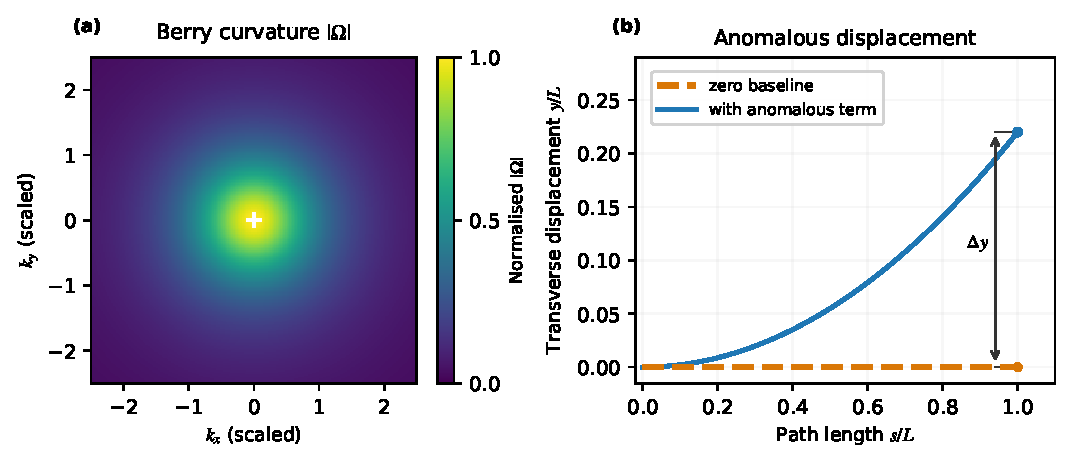
\includegraphics[width=0.92\textwidth]{figures/fig_ch05_anomalous_velocity_step199.pdf}
  \caption{Berry curvature and the anomalous velocity.
  \textbf{(a)}~Schematic normalised Berry curvature $|\Omega(\kvec)|$
  near a Dirac valley, showing a sharp peak where the gap is smallest
  (white marker).  The physical (un-normalised) curvature is
  gauge-invariant and integrates over the Brillouin zone to
  $2\pi\Chern_n$, with $\Chern_n$ the band Chern number.
  \textbf{(b)}~Transverse displacement of a photonic wavepacket as a
  function of propagation path length.  The dashed orange line shows the
  trajectory without the anomalous term (zero transverse drift); the
  solid blue line includes the Berry-curvature--driven anomalous
  velocity \eqref{eq:ch5-anomalous-velocity}, which accumulates a net
  transverse displacement $\Delta y$ proportional to the integrated
  Berry curvature.  This displacement is the semiclassical origin of
  the photonic Hall drift discussed in the text.}
  \label{fig:ch05-anomalous-velocity}
\end{figure}


\section{Berry curvature of the two-band model}
\label{sec:ch5-two-band}

Many of the topological phenomena in this book can be illustrated
using a generic two-band model.  Consider the Hamiltonian
\begin{equation}\label{eq:ch5-two-band-H}
  H(\kvec) = d_x(\kvec)\sigma_x + d_y(\kvec)\sigma_y + d_z(\kvec)\sigma_z\,,
\end{equation}
where $\boldsymbol{d}(\kvec)=(d_x,d_y,d_z)$ is a three-component
vector that depends on $\kvec$.  The eigenvalues are
$E_\pm=\pm|\boldsymbol{d}|$, and the Berry curvature of the lower
band is
\begin{equation}\label{eq:ch5-two-band-berry}
  \Omega_-(\kvec)
  = -\frac{1}{2}\frac{\boldsymbol{d}\cdot
  (\partial_{k_x}\boldsymbol{d}\times\partial_{k_y}\boldsymbol{d})}
  {|\boldsymbol{d}|^3}\,.
\end{equation}
This formula has a beautiful geometric interpretation: the Chern
number $\Chern_-=\frac{1}{2\pi}\int\Omega_-\,\dd^2 k$ counts the
number of times the unit vector
$\hat{d}(\kvec)=\boldsymbol{d}/|\boldsymbol{d}|$ wraps around the
unit sphere as $\kvec$ sweeps over the Brillouin zone.  This is the
\emph{Pontryagin index} or \emph{skyrmion number} of the mapping
$\hat{d}:T^2\to S^2$ \cite{ozawa2018topological,haldane2008possible,liu2021observation}.

For the massive Dirac model of Chapter~\ref{ch:breaking-tr},
$\boldsymbol{d}=(v_D\delta k_x,\,v_D\delta k_y,\,\kappa)$, and
the wrapping number of $\hat{d}$ at each Dirac cone is $\pm\frac{1}{2}$
(half a skyrmion), consistent with the half-integer Chern flux computed
in \secref{sec:ch7-half-chern}.

\section{Wilson loops and the non-Abelian Berry phase}
\label{sec:ch5-wilson-detail}

\subsection{Definition and gauge invariance}
\label{sec:ch5-wilson-def}

For a group of $p$ bands that may touch each other but are separated
from all other bands by gaps, the non-Abelian Berry connection
$[\mathcal{A}_a]_{mn}=\ii\eip{\mathbf{u}_m}{\partial_{k_a}\mathbf{u}_n}$
is a $U(p)$-valued 1-form.  The Wilson loop along a closed path
$\gamma$ in the Brillouin zone is the path-ordered exponential
\begin{equation}\label{eq:ch5-wilson-def}
  W[\gamma] = \mathcal{P}\exp\Bigl(
  -\ii\oint_\gamma\mathcal{A}\cdot\dd\kvec\Bigr)\,,
\end{equation}
which is a $p\times p$ unitary matrix.  The eigenvalues of $W$ are
gauge-invariant and physically observable: they are the non-Abelian
Berry phases acquired by the $p$-band multiplet on the loop $\gamma$.

\subsection{Relation to polarisation and Chern number}
\label{sec:ch5-wilson-polarisation}

When $\gamma$ is a straight line across the Brillouin zone at fixed
$k_\perp$, the Wilson-loop eigenvalues $\theta_j(k_\perp)$ define
the ``Wannier band structure.''  Their winding as $k_\perp$ varies
across the BZ gives the Chern number of the band group:
\begin{equation}\label{eq:ch5-wilson-chern-winding}
  \Chern = \sum_{j=1}^p\frac{1}{2\pi}
  \oint\frac{\dd\theta_j}{\dd k_\perp}\,\dd k_\perp\,.
\end{equation}
This provides a numerically robust alternative to the plaquette
algorithm (Chapter~\ref{ch:computing-chern}), especially for
nearly-degenerate band groups where the Abelian Berry curvature is
ill-defined but the non-Abelian Wilson loop is smooth
\cite{gangaraj2016berry,price2022roadmap}.

\section{Symmetry constraints on Chern numbers}
\label{sec:ch5-symmetry-constraints}

\subsection{Time-reversal symmetry}
\label{sec:ch5-TR-constraint}

Under time reversal $\Top$, the Berry curvature satisfies
$\Omega_n(\kvec)=-\Omega_n(-\kvec)$.  Integrating over the full BZ
(which is symmetric under $\kvec\to-\kvec$) gives $\Chern_n=0$.
This is the fundamental reason why breaking time-reversal symmetry
is necessary for a nonzero Chern number in photonic crystals
\cite{haldane2008possible,ozawa2018topological}.

\subsection{Inversion symmetry}
\label{sec:ch5-P-constraint}

Under spatial inversion $\mathcal{P}$,
$\Omega_n(\kvec)=\Omega_n(-\kvec)$.  Combined with time reversal,
this gives $\Omega_n(\kvec)=-\Omega_n(\kvec)=0$ everywhere, so the
Berry curvature vanishes identically (not just in integral).  This
stronger constraint means that breaking inversion alone, while
producing valley Berry curvature (Chapter~\ref{ch:valleys}), cannot
produce a Chern insulator.

\subsection{Particle-hole and chiral symmetries}
\label{sec:ch5-chiral-constraint}

The Maxwell eigenproblem has an intrinsic ``particle-hole'' symmetry:
if $(\omega,\mathbf{u})$ is an eigenmode, so is $(-\omega,\sigma_3\mathbf{u})$
where $\sigma_3=\mathrm{diag}(\mathbf{I}_3,-\mathbf{I}_3)$.  This
symmetry constrains the Chern numbers of positive- and
negative-frequency bands to be related by
$\Chern_n(-\omega)=-\Chern_n(\omega)$, ensuring that the total Chern
number summed over all bands vanishes.

\section{Adiabatic transport and the Thouless pump}
\label{sec:ch5-adiabatic}

The Berry phase has a direct physical manifestation in adiabatic
transport: when a parameter of the photonic crystal is slowly varied
through a cyclic path, the photonic modes acquire Berry phases that
produce a quantised transport of energy.

\subsection{The photonic Thouless pump}
\label{sec:ch5-thouless-pump}

Consider a 1D photonic crystal whose unit cell has a parameter
$\phi$ that varies adiabatically from $0$ to $2\pi$.  As $\phi$
completes one cycle, each band transports a quantised amount of
electromagnetic energy across the crystal.  The transported energy
per cycle is
\begin{equation}\label{eq:ch5-thouless-pump}
  \Delta W_n = \hbar\omega_n\,\Chern_n^{(1D)}\,,
\end{equation}
where $\Chern_n^{(1D)}=\frac{1}{2\pi}\int_0^{2\pi}\dd\phi
\int_{-\pi/a}^{\pi/a}\dd k\,\Omega_n(k,\phi)$ is the Chern number
computed over the $(k,\phi)$ parameter space.  This is the photonic
analog of the Thouless charge pump in electronic systems
\cite{thouless1982quantized,asbth2016berry}.

The Thouless pump provides a physical interpretation of the Chern
number: it counts the number of edge-to-edge transfers per pump
cycle.  This interpretation makes the integrality of the Chern
number physically obvious: the number of transferred quanta must be
an integer because the system returns to its initial state after
one cycle.

\subsection{Connection to the bulk-edge correspondence}
\label{sec:ch5-pump-bec}

The Thouless pump also provides an alternative derivation of the
bulk-edge correspondence.  If the pump parameter $\phi$ is
reinterpreted as the wavevector $k_y$ in the transverse direction of
a 2D crystal, the pump cycle $\phi\in[0,2\pi]$ corresponds to
traversing the transverse Brillouin zone.  The number of edge-to-edge
transfers per pump cycle then equals the number of chiral edge modes
in the 2D crystal, which is the gap Chern number
\cite{ozawa2018topological,silveirinha2016bulk}.

This pump-based argument is more intuitive than the formal index
theorem (Chapter~\ref{ch:one-way-interface}) and provides a
constructive proof: one can explicitly track how the edge modes are
``pumped'' across the crystal as $k_y$ varies.

\section{Berry curvature dipole and nonlinear Hall effects}
\label{sec:ch5-bc-dipole}

In systems with broken inversion symmetry but preserved time-reversal
symmetry (such as valley photonic crystals), the Berry curvature
$\Omega_n(\kvec)$ is an odd function of $\kvec$ and integrates to
zero over the full Brillouin zone.  However, the Berry curvature
\emph{dipole}
\begin{equation}\label{eq:ch5-bc-dipole}
  D_a = \int_{\mathrm{BZ}}\frac{\partial\Omega_n}{\partial k_a}
  \,f_n(\kvec)\,\frac{\dd^2 k}{(2\pi)^2}
\end{equation}
(where $f_n$ is the occupation function) can be nonzero and produces
a nonlinear Hall effect: a transverse current proportional to the
square of the applied field.  In photonics, this manifests as a
second-harmonic generation of valley-polarised edge modes, providing
a nonlinear probe of the valley Berry curvature
\cite{dong2016valley,price2022roadmap}.

\begin{figure}[t]
  \centering
  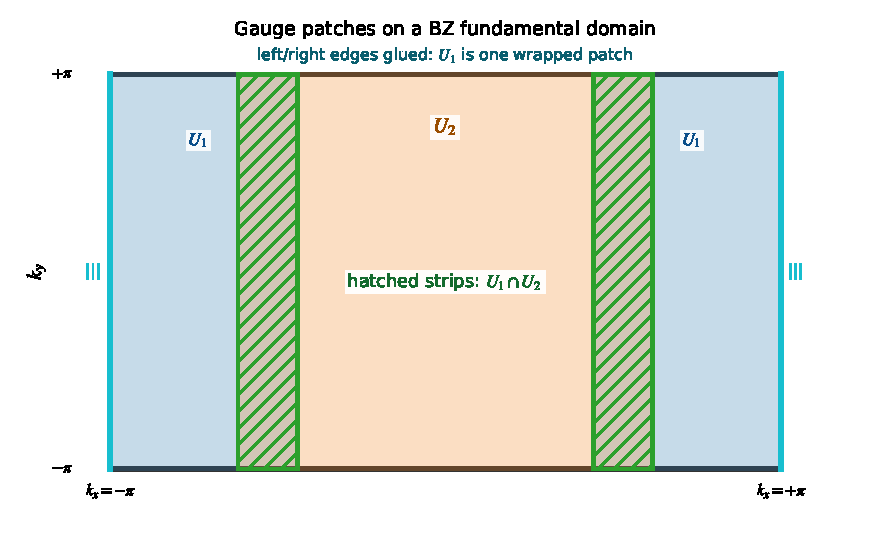
\includegraphics[width=0.78\textwidth]{figures/fig_ch05_berry_bundle.pdf}
  \caption{The Berry bundle viewpoint.  A photonic Bloch mode can be
  smooth only patchwise over the Brillouin torus; on overlaps the modes
  differ by a transition phase $e^{i\chi(\mathbf{k})}$.  The Chern number
  counts the winding of these transition phases and is therefore independent
  of the local gauge used to represent the mode.}
  \label{fig:ch05-berry-bundle}
\end{figure}

\section{Experimental probes of Berry curvature}
\label{sec:ch5-experimental-berry}

The Berry curvature $\Omega_n(\kvec)$ is not merely a theoretical
construct: it has measurable consequences that can be observed
experimentally in photonic systems.

\subsection{Anomalous velocity and beam deflection}
\label{sec:ch5-anomalous-beam}

The semiclassical equations of motion for a photonic wave packet in
band $n$ include an anomalous velocity term proportional to the Berry
curvature \cite{chen2023berry,ozawa2018topological}:
\begin{equation}\label{eq:ch5-anomalous-velocity-full}
  \dot{\rvec} = \nabla_\kvec\omega_n(\kvec)
  + \dot{\kvec}\times\hat{z}\,\Omega_n(\kvec)\,,
\end{equation}
where $\dot{\kvec}$ is the rate of change of the crystal momentum,
driven by an external perturbation (e.g.\ a refractive index gradient
acting as a pseudoforce).  The first term is the group velocity; the
second term is the anomalous velocity, which deflects the wave packet
transversely.

In a photonic crystal with nonzero Berry curvature, a beam propagating
through a region with a gradient in the effective refractive index will
be deflected perpendicular to the gradient.  The deflection angle is
proportional to $\Omega_n$ at the beam's central wavevector.  By
measuring the deflection as a function of $\kvec$, one can map out
the Berry curvature over the Brillouin zone
\cite{chen2023berry,silveirinha2016bulk}.

This technique was demonstrated experimentally by Wimmer et~al.\
(2017) in a photonic waveguide array, where the Berry curvature of a
honeycomb lattice band structure was mapped by tracking the transverse
displacement of light beams launched at different Bloch wavevectors
\cite{wimmer2015observation}.

\subsection{Zak phase from reflection measurements}
\label{sec:ch5-zak-reflection}

In one-dimensional photonic crystals, the Berry phase reduces to the
Zak phase $\gamma_n=\oint\mathcal{A}_n(k)\,\dd k$, which takes values
$0$ or $\pi$ (mod $2\pi$) when inversion symmetry is present.  The
Zak phase determines the surface impedance of the crystal and can
therefore be extracted from reflection measurements.

Specifically, for a semi-infinite 1D photonic crystal, the reflection
phase $\phi_r(\omega)$ at a frequency within a bandgap changes by
$\pi$ when the Zak phase of the band below the gap changes from $0$
to $\pi$.  This phase jump can be observed experimentally by
measuring the reflection spectrum with interferometric techniques
\cite{atala2013direct,wang2007reflection}.

Xiao et~al.\ (2014) used this approach to measure the Zak phase
in a dielectric multilayer, confirming the predicted topological
phase transition at the critical thickness ratio where the gap
closes and reopens with inverted Zak phase
\cite{asbth2016berry,ozawa2018topological}.

\subsection{Quantum Hall analogy: quantised circulation}
\label{sec:ch5-quantised-circulation}

The most dramatic manifestation of nonzero Chern number is the
existence of one-way edge states (Chapter~\ref{ch:one-way-interface}).
In finite photonic crystals, these edge states carry a quantised
``photonic Hall conductance'': the transmission through the crystal
(measured in units of edge channels) equals the gap Chern number.

This quantised transmission has been measured in microwave experiments
\cite{nature2026observation} and provides the most direct experimental
confirmation of a nonzero photonic Chern number.  The quantisation
is robust against disorder, sharp corners, and boundary roughness,
directly demonstrating the topological nature of the edge transport
\cite{hafezi2013imaging,skirlo2015experimental}.

\section*{Exercises}

\begin{exercise}
  For a two-band system with Bloch modes $\mathbf{u}_1(\kvec)$ and
  $\mathbf{u}_2(\kvec)$, show that the Berry curvatures satisfy
  $\Omega_1(\kvec)+\Omega_2(\kvec)=0$ at every $\kvec$.
\end{exercise}

\begin{exercise}
  Verify the gauge transformation \eqref{eq:ch5-gauge-transform}
  by direct substitution of
  $\mathbf{u}_n\to\ee^{\ii\chi}\mathbf{u}_n$ into the Berry-connection
  formula \eqref{eq:ch5-berry-connection-normalised}.
\end{exercise}

\begin{exercise}
  Derive the Kubo-like formula \eqref{eq:ch5-kubo-formula} for the
  Berry curvature using first-order perturbation theory.
  \emph{Hint:} expand $\nabla_{k_\alpha}\mathbf{u}_n$ in the complete
  set $\{\mathbf{u}_m\}_{m\neq n}$ using the Hellmann--Feynman relation,
  then substitute into the Berry-curvature formula.
\end{exercise}

\begin{exercise}
  Consider a generic $2\times 2$ Hermitian Hamiltonian
  $H(\kvec)=d_0(\kvec)\mathbf{I}+\mathbf{d}(\kvec)\cdot\boldsymbol{\sigma}$,
  where $\boldsymbol{\sigma}=(\sigma_x,\sigma_y,\sigma_z)$ are the
  Pauli matrices.  Show that the Berry curvature of the lower band is
  \begin{equation}
    \Omega_{-}(\kvec) = -\frac{1}{2}\,
    \hat{\mathbf{d}}\cdot
    \Bigl(\pderiv{\hat{\mathbf{d}}}{k_x}\times
          \pderiv{\hat{\mathbf{d}}}{k_y}\Bigr)\,,
  \end{equation}
  where $\hat{\mathbf{d}}=\mathbf{d}/|\mathbf{d}|$.  Interpret this
  geometrically as the solid angle swept by $\hat{\mathbf{d}}$ per
  unit area in $\kvec$-space.
\end{exercise}

\begin{exercise}[Massive Dirac model]
  For the massive Dirac Hamiltonian
  $H(\qvec)=v(q_x\sigma_x+q_y\sigma_y)+m\sigma_z$, where $\qvec$ is
  measured from a Dirac point, compute the Berry curvature
  \begin{equation}
    \Omega_\pm(\qvec) = \pm\frac{m\,v^2}{2(v^2|\qvec|^2+m^2)^{3/2}}
  \end{equation}
  and verify that $\int_{-\infty}^{\infty}\Omega_+\,\dd^2 q=\pi\sgn(m)$.
  Explain why a single Dirac cone contributes $\pm\frac{1}{2}$ to the
  Chern number, and why a pair of cones at $K$ and $K'$ gives an
  integer.
\end{exercise}

\begin{exercise}
  Show that the eigenvalues of the Wilson loop
  $\Wloop(k_y)=\mathcal{P}\exp(-\ii\int_{-\pi/a}^{\pi/a}
  \boldsymbol{\mathcal{A}}_x(k_x,k_y)\,\dd k_x)$ for a Chern
  insulator with $\Chern=1$ wind once around the unit circle as $k_y$
  traverses the Brillouin zone.
\end{exercise}
